%!TEX root = ../dokumentation.tex

\chapter{Medizinische Grundlagen}

\section{Herzparameter}
Das menschliche Herz kann mit vielen verschiedenen Werten parametrisiert werden. Der wohl bekannteste Parameter ist dabei die Herzfrequenz (Hf). Sie gibt an, wie oft das Herz in einer bestimmten Zeit schlägt. Meist wird dafür das Zeitintervall einer Minute gewählt und die in dieser Zeit gemessenen Herzschläge in der Einheit \emph{bpm} (beats per minute) angegeben. 

Die Herzfrequenz ist abhängig von verschiedenen Faktoren. So spielen beispielsweise Alter und körperliche Fitness eine große Rolle. Bei trainierten (Ausdauer) Sportlern schlägt das Herz in Ruhe bedeutend seltener als bei untrainierten Personen. Dies kann damit erklärt werden, dass durch das Ausdauertraining das \textbf{Schlagvolumen (SV)} erhöht werden kann. Das Schlagvolumen gibt an, wie viel Blut das Herz mit einem Schlag durch den Körper pumpen kann. Wenn sich dieses Volumen also erhöht, muss das Herz seltener schlagen, um das \textbf{Herzminutenvolumen (HMV)} zu halten. Dieses berechnet sich aus Herzfrequenz und Schlagvolumen:
\begin{equation}\formelentry{Herzminutenvolumen (HMV)}
	%Herzminutenvolumen = Herzfrequenz * Schlagvolumen
	HMV = Hf * SV
\end{equation} 
Bei körperlicher Belastung, beispielsweise sportlicher Aktivität, erhöht sich das benötigte Herzminutenvolumen, da die Muskeln mehr Sauerstoff brauchen. Da sich das Schlagvolumen des Herzens nicht anpassen lässt, erhöht sich die Herzfrequenz um dem benötigten Herzminutenvolumen gerecht zu werden. Grundsätzlich, wie jeder bei sich selber feststellen kann, erhöht sich die Herzfrequenz bei körperlicher Aktivität. Durch sehr starker Aktivität kann die Herzfrequenz auf ein Maximum ansteigen. Die maximale Herzfrequenz kann mit folgender Faustformel abgeschätzt werden: 
\begin{equation}\formelentry{Maximale Herzfrequenz}
	%maximale Herzfrequenz = 220 - Alter
	Hf_{max} = 220 - Alter
\end{equation}
gesprochen. Allerdings muss zwischen Puls und Herzfrequenz unterschieden werden, da diese nicht identisch sind. 
Die Herzfrequenz beschreibt, wie bereits in den vorhergehenden Abschnitten beschrieben, die tatsächlichen Schläge des Herzens. Zur Messung der Herzfrequenz kann ein EKG genutzt werden,
Der \textbf{Puls} hingegen wird peripher, beispielsweise am Hals oder Handgelenk gemessen. Dabei werden Pulswellen erfasst, welche sich durch den Körper bewegen. Eine Pulswelle entsteht wenn das Herz schlägt, und das Blut durch den Körper pumpt. Dabei wird das Blut gegen die Arterienwände gedrückt und eine Pulswelle kann detektiert werden.
Bei gesunden Menschen entspricht der Puls der Herzfrequenz, da jeder Herzschlag Blut durch den Körper pumpt und somit auch eine messbare Pulswelle erzeugt. Bestimmte Herzrhythmuskrankheiten können dafür verantwortlich sein, dass Puls und Herzfrequenz voneinander abweichen. Dabei können Kontraktionen des Herzens entstehen, welche kein oder nicht genug Blut durch den Körper pumpen um eine messbare Pulswelle zu erzeugen. Die Differenz zwischen Herzfrequenz und Puls nennt sich \textbf{Pulsdefizit} (und ist bei gesunden Menschen 0).

Die Variation der Herzfrequenz wird über das \textbf{vegetative Nervensystem} geregelt. Dies besteht aus dem \textit{Sympathikus} und seinem Gegenspieler, dem \textit{Parasympathikus}. Außerdem ist das \textit{enterische Nervensystem (Eingeweidenervensystem)} teil des vegetativen Nervensystems. Dies spielt für die Steuerung des Herzens allerdings keine Rolle und wird daher im Laufe dieser Arbeit nicht mehr erwähnt. Ebenso haben Sympathikus und Parasympathikus Funktionen in der Verdauung. Da dies ebenfalls keine Relevanz für das Herz hat, wird darauf nicht weiter eingegangen. Die Folgende Erklärung von Sympathikus und Parasympathikus beziehen sich daher nur auf die für das Herz relevanten Eigenschaften.

\begin{enumerate}
	\item \textbf{Sympathikus} 
	
	Der Sympatikus kann den Organismus auf eine Aktivitätssteigerung ("fight or fligt") einstellen. Er ist der dominante Teil des vegetativen Nervensystems, wenn es um Stresssituationen geht. Wenn diese eintritt, wird die Aktivität von situationsbedingt unwichtigen Organen, beispielsweise Darm oder andere Organe die zur Verdauung beitragen, gesenkt. 
	Die Aktivität von Organen die in Stresssituationen wichtig sind wird verstärkt. So werden beispielsweise die Pupillen vergrößert.
	\color{red}Die Herzfrequenz wird stark erhöht.\color{black}
	
	\item \textbf{Parasympathikus}
	
	Der Parasympathikus stellt den Organismus auf Ruhesituationen ("rest and digest") ein. So werden in den dominanten Phasen des Parasympathikus Organe mit Verdauungsfunktionen in ihrer Aktivität gestärkt. Der Körper wird auf Entspannung und Regeneration heruntergefahren. 
	\color{red}Die Herzfrequenz wird in diesen Phasen stark gesenkt.\color{black}
\end{enumerate}

Das vegetative Nervensystem ist in seiner Funktion \textbf{unwillkürlich}. Das bedeutet, es kann nicht bewusst von der jeweiligen Person gesteuert werden. Dadurch sind Messungen, beispielsweise an der Herzfrequenz sehr gut geeignet, um bestimmte äußere Einflüsse zu untersuchen.
Die Ergebnisse können nicht von der Testperson verfälscht werden, da sie das vegetative Nervensystem nicht beeinflussen kann. (Andere äußere Einflüsse wie Aufregung müssen berücksichtigt werden und können das Ergebnis logischerweise verfälschen.)
		
\color{red} Um nun den konkreten Einfluss von elektromagnetischen Wellen zu Untersuchen kann die Herzfrequenz als Messparameter benutzt werden. Ein weiterer Parameter welcher stark abhängig vom vegetativen Nervensystem ist, ist die \textbf{Herzfrequenzvariabilität (HRV)}. Im Verlauf dieser Arbeit, wird die Herzratenvariabilität als entscheidender Parameter genutzt. Alle durchgeführten Messungen und daraus abgeleiteten Interpretationen beziehen sich auf diese. 
\color{black}

\section{Herzfrequenzvariabilität (HRV)}

Die Herzfrequenzvariabilität, auch Herzratenvariabilität ist die zeitliche Variation zwischen zwei aufeinanderfolgenden Herzschlägen \color{red}wiki?\color{black}.

\begin{figure}[!htbp]
    \centering
    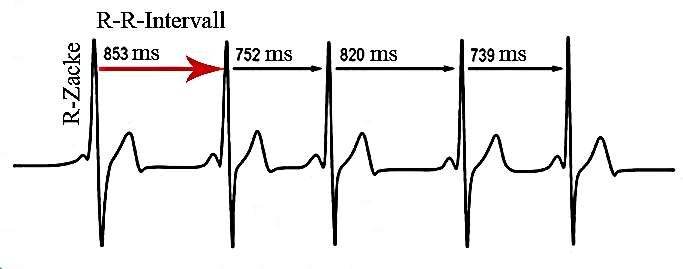
\includegraphics[width=0.7\linewidth]{RR}
    \caption{R-R-Intervall}
    \label{fig:R-R-Intervall}
\end{figure}

In dieser Grafik ist eine EKG Messung zu sehen. Gut erkennbar sind die hohen R Zacken. Diese werden benutzt, um die Herzfrequenzvariabilität zu berechnen. Dabei wird die Zeit zwischen zwei Herzschlägen als die Zeit zwischen den aufeinanderfolgenden R-Zacken definiert. In diesem Schaubild liegt diese Zeit, also das R(-)R-Intervall zwischen 739 ms und 853 ms. Das RR-Intervall wird in der Literatur oft als NN-Intervall bezeichnet. Der Begriff RR wird auch bei Messen des Blutdrucks verwendet. Dort steht RR für \textit{Riva-Rocci}. Um eine Verwechslung zu vermeiden, wird daher im Kontext der HRV vom NN-Intervall gesprochen.




\section{Listings}
\subsection{lorem listum}

\begin{lstlisting}[caption={Einbinden von Code aus externer Datei mit Angabe eines Zeilenbereichs},label=inputFromFile]
\lstinputlisting[language=Python,firstline=37,lastline=45]{source_filename.py}
\end{lstlisting}

\blindmathpaper

\begin{lstlisting}[caption=Dies ist ein Listing,label=lstcode]
for i:=maxint to 0 do
begin
{ do nothing }
end;
Write('Case insensitive ');
Write('Pascal keywords.');
\end{lstlisting}

\begin{figure}[ht]%
	\centering
	\begin{circuitikz}
		\draw (0,0)
				to[V,v=$U_q$] (0,2)
				to[R=$R_1$] (2,2)
				to[short] (6,2)
				to[R=$R_2$] (6,0)
				to[short] (0,0);
	\end{circuitikz}
	\caption{Elektrische Schaltung - ein Beispiel}%
\end{figure}
